\documentclass[fontsize=11pt]{article} 
\usepackage[spanish]{babel} 
\usepackage[total={6in, 8in}]{geometry}
\usepackage{amsmath,amsfonts,amsthm} 
\usepackage{graphicx}
\usepackage{float}
\usepackage{enumerate} 
\usepackage{pdflscape}
\usepackage{stackrel}
\usepackage{babel}
\graphicspath{ {images/} }
\usepackage{hyperref}
\usepackage{lscape}
\usepackage[utf8]{inputenc}
\title{Proyecto Demografía Matemática}
\author{  López Hernández Alejandro $|$ Montoya Franco Luis Angel} % Your name
\date{\normalsize\today} % Today's date or a custom date
\begin{document}
\begin{titlepage}
	\centering
	
\includegraphics[width=0.15\textwidth]{UNAM}\par\vspace{1cm}
	{\scshape\LARGE Universidad Nacional Autónoma de México\par}
	\vspace{1cm}
	{\scshape\Large Facultad de Estudios Superiores Acatlán\par}
	\vspace{1.5cm}
	{\huge\bfseries Estudio demográfico de Chihuahua y consecuencias de los homicidios  \par}
	\vspace{2cm}
	{\scshape\Large Demografía Matemática\par}
	\vspace{2cm}
	{\Large\itshape López Hernández Alejandro \\ Montoya Franco Luis Angel\par}
	\vfill
	Profesor\par
	Ramos López Aram Isai

	\vfill

% Bottom of the page
	{\large \today\par}
\end{titlepage}
%\begin{abstract}
 %  El objetivo de este proyecto es usar datos poblacionales del estado de Chihauhua para analizarlos y a partir del analisis poder corregirlos y estudiar la estructura poblacional, posteriormente usando las defunciones durante el año 2015 en Chihuahua causadas por agresiones, estimar el efecto que tienen sobre nuestra población ($_u AV_{j}$). 
%\end{abstract}

\section*{Introducción}
 El estudio de la población humana resulta de gran ayuda para poder mejorar la calidad de vida, por ejemplo, puede mostrarnos zonas geográficas donde la tasa de mortalidad es mayor, y a su vez podría deberse a una enfermedad que afecta a esa localidad. 
Por esta razón y entre otras es importante conocer la población y todos los factores que la afectan. 
\\Por consiguiente el propósito de este proyecto es analizar la población del estado de Chihuahua y además determinar como los homicidios que ocurren en este han afectado la esperanza de vida de sus habitantes.
El motivo por el que se estudiara el estado de Chihuahua es porque en él se encuentra Ciudad Juárez la cual es conocida por ser una ciudad con altos índices delictivos, de los cuales destaca el homicidio. 
\\ 
\section*{Distribución de la población.}
	Comenzaremos con analizando cómo se distribuye la población por edad, esto es importante pues de esta forma podemos observar en que edades se concentra el mayor y menor volumen de población. Para poder realizar esto, se extrajo la población de Chihuahua de la página oficial de la CONAPO en la cual ya está desagregada por edades. 
\\Debido a que el rango de edades de la población es bastante grande, resulta difícil notar que edades concentran un mayor número de habitantes por lo que, de forma de ayuda, presentamos la pirámide poblacional del estado de Chihuahua.

\begin{figure}[H]
\centering
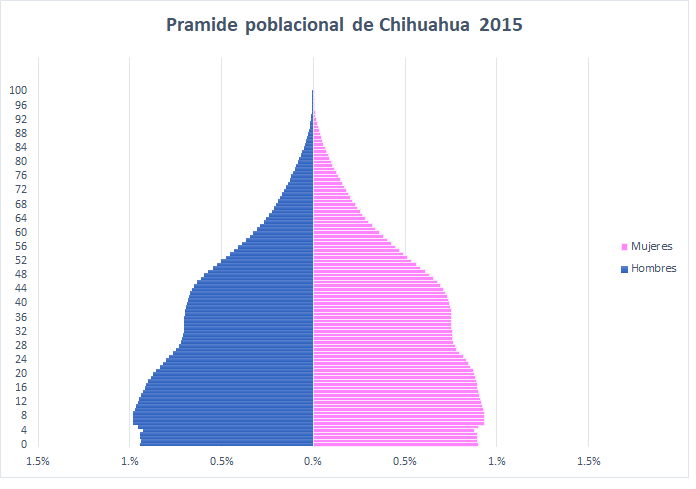
\includegraphics[width=0.6\textwidth]{Piramide}
%\caption{Muertes por agresiones en Chihuahua distribuidas por municipio}
\end{figure}

\\Podemos observar que la base de la pirámide es la parte más ancha de esta, indicando así que la mayor parte de la población está concentrada en edades jóvenes, aproximadamente de los 0 a los 20 años cumplidos lo cual nos da un indicio de que Chihuahua se encuentra en desarrollo, pues los jóvenes cuentan con el potencial de convertirse en un factor importante para la economía del estado.
\section*{Desegregación y preferencia al declarar edades}
\\Como vimos en la sección anterior la mayoría de la población era joven, pero ¿Sera esto verdad? Es decir, no todo declaran su edad correctamente, como bien se sabe, mucha gente tiende redondear su edad a dígitos que terminen en cero o cinco, ya sea para aumentar o disminuir su edad real. 
\\Para poder darnos una idea de este efecto sobre la población de Chihuahua utilizaremos el índice de Whipple, el cual es un indicador de que tanta es la preferencia hacia un digito en las edades, el cual funciona comparando las poblaciones de las edades terminadas en dicho digito que se quiere estudiar dividido entre las poblaciones que se cree que declaran correctamente su edad, las cuales abarcan de los 23 a los 62 años, multiplicado por una constante    (usualmente 100) y divido entre la proporción de edades terminadas en el digito a estudiar. A si en Indicé de Whipple para el digito cero se calcula como:
\[
Iw_{0}=\frac{P_{30}+P_{40}+P_{50}+P_{60}}{\frac{\stackrel[i=23]{62}{\sum}P_{i}}{10}}\times100
\]

Por lo que $$Iw_0 =94.3$$ 
Análogamente para las edades terminadas en digito 5 tenemos: $$Iw_5=105.8$$

Estos resultados indican que hay un rechazo hacia el digito cero y una atracción hacia el cinco.
También podemos calcular el índice para edades terminadas en cero y cinco a la vez. De la siguiente manera:

\[
Iw_{0,5}=\frac{P_{30}+P_{40}+P_{50}+P_{60}+P_{25}+P_{35}+P_{45}+P_{55}}{\frac{\stackrel[i=23]{62}{\sum}P_{i}}{10}}\times100
\]
Del cual resulta $$Iw_{0,5} =100.084$$

\\El cual, nos dice que la declaración de edades hacia el digito 0 y 5 en promedio no tiene preferencia, lo cual resulta paradójico a los dos anteriores, pero esto es solo por que como uno de los dígitos atrae y el otro rechaza (como indicaban los dos índices pasados) se inhibe el efecto entre estos.
 
\\Finalmente veremos la eficacia de interpolación osculatoría con el método de Beers, pues la mayoría de las poblaciones, son publicadas en grupos quinquenales, y regularmente es necesario interpolar para ver la población desagregada por edades. En este caso, ya contamos con la Población desagregada por edad, por lo que la agruparemos en grupos quinquenales y usaremos la interpolación antes mencionada, para a continuación calcular el error cuadrático promedio de todas las estimaciones. 
El EMC (error cuadrático medio) se calcula de la siguiente forma:

$$EMC=\frac{1}{n} \sum_{i=1}^n (O_{i}-Ô_{i})^2$$

Donde $Ô_i$ es el valor estimado (el arrojado por la interpolación) y $O_{i}$ el valor real que tomo la población de edad i. A si 

$$EMC=3,406,570$$

\\Calculando la raíz del EMC obtenemos 1,846 que se puede interpretar como el promedio de personas que se pierde por edad, lo cual, en edades donde el volumen de población es grande, podría decirse que insignificante ese error, sin embargo en las edades avanzadas que son las que tiene menor población es un error inmenso pues resulta ser incluso el 200\% de la población de algunas de esas edades. 
\\NOTA: Para profundizar en los valores obtenidos en la interpolación de Beers, pueden consultar el archivo Excel adjunto a este documento, donde se observan todos los valores obtenidos.


\section*{Impacto de los homicidios en la esperanza de vida}
Como bien se sabe se tiene un gran problema de homicidios en el estado de Chihuahua, durante el año 2015 se reportaron\cite{DAT} 1535 homicidios en total, estos en su mayoría en Juarez (440), por la gran extensión del estado de Chihuahua, los homicidios se concentran en zonas muy particulares como se muestra en el siguiente mapa: 
\begin{figure}[H]
\centering
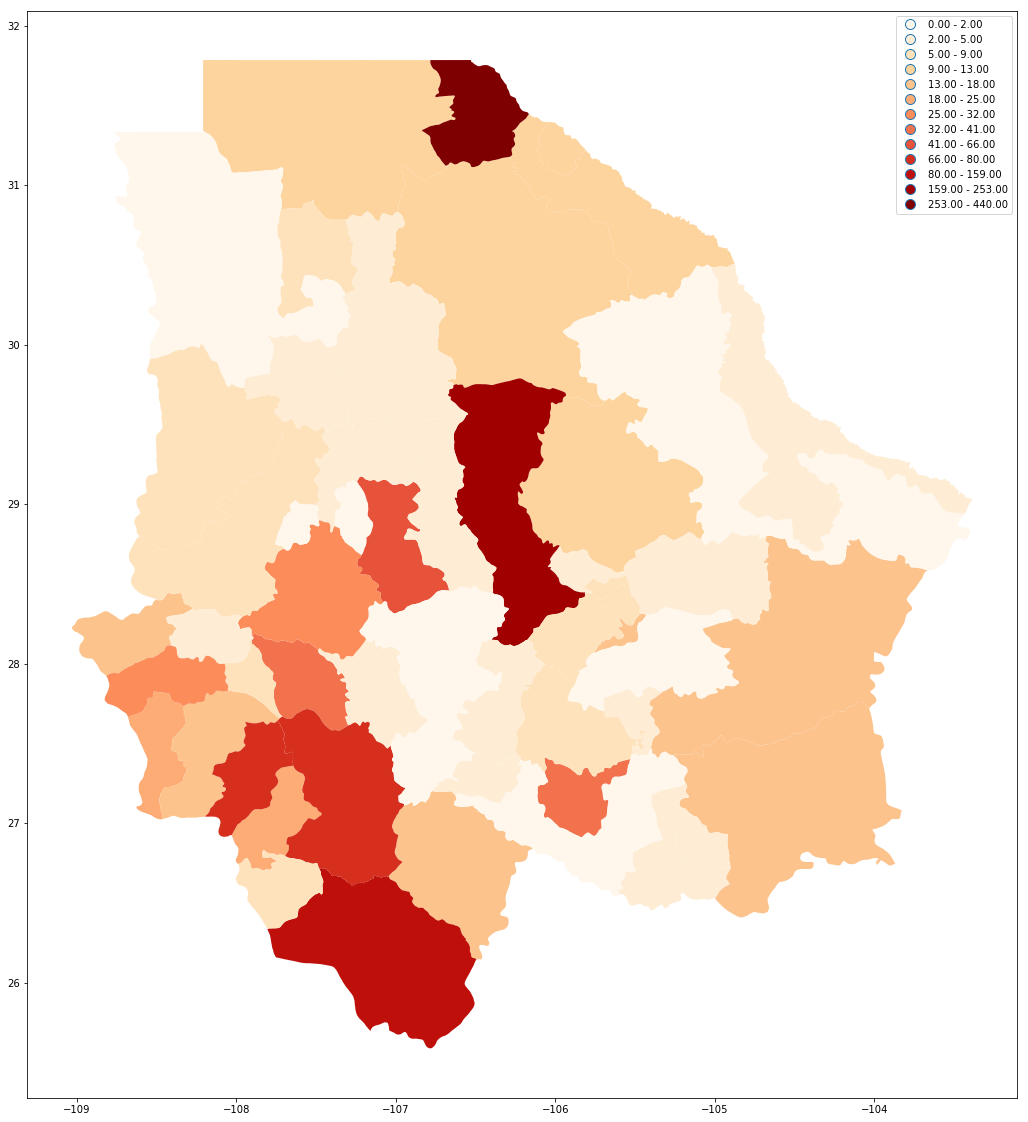
\includegraphics[width=0.4\textwidth]{map}
\caption{Muertes por agresiones en Chihuahua distribuidas por municipio}
\end{figure}
Como se esperaría el numero de homicidios es mayor en los hombres en edades principalmente de 15 a 50 años, mientras que en las mujeres ocurren principalmente en edades de 20 a 45 años, la información se encuentra detallada en la siguiente tabla y gráfica: 

\begin{table}[H]
\centering

\begin{tabular}{|c|c|c|}
\hline
Edad  & Hombres & Mujeres \\ \hline
0     & 2       & 1       \\ \hline
1-4   & 8       & 2       \\ \hline
5-9   & 4       & 2       \\ \hline
10-14 & 11      & 6       \\ \hline
15-19 & 136     & 9       \\ \hline
20-24 & 213     & 20      \\ \hline
25-29 & 227     & 26      \\ \hline
30-34 & 173     & 19      \\ \hline
35-39 & 185     & 14      \\ \hline
40-44 & 162     & 19      \\ \hline
45-49 & 102     & 6       \\ \hline
50-54 & 61      & 3       \\ \hline
55-59 & 38      & 7       \\ \hline
60-64 & 28      & 2       \\ \hline
65-69 & 17      & 3       \\ \hline
70-74 & 13      & 1       \\ \hline
75-79 & 10      & 1       \\ \hline
80-84 & 5       & 1       \\ \hline
\end{tabular}
\caption{Muertes por agresiones en Chihuahua durante 2015}
\end{table}
\label{my-label}
\begin{figure}[H]
\centering
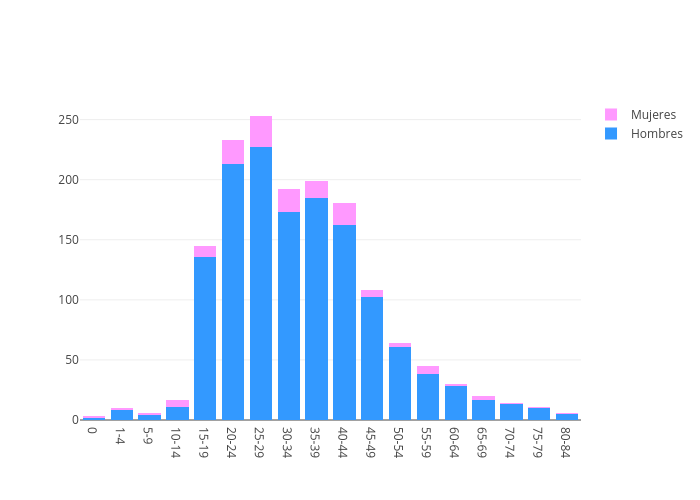
\includegraphics[width=0.7\textwidth]{homihist}
\caption{Histograma de homicidios separado por hombres y mujeres}
\end{figure}

Para poder cuantificar el efecto que tuvieron exclusivamente estos homicidios utilizaremos el indice $_0AP_j$ (Años de vida perdidos por la causa de defunción $j$ desde la edad $0$) propuesto por Arriaga\cite{ARR} donde se supone lo siguiente: 
\begin{enumerate}[a)]
        \item Suponer que la mortalidad debería ser nula entre dos edades
elegidas para el análisis. Vaie decir, aquellos que mueren
deberían haber vivido hasta la edad superior del intervalo de
edades donde se analiza la mortalidad.
        \item Suponer que entre las dos edades elegidas para el análisis,
aquellos que mueren a una edad determinada, de no haber
muerto, deberían haber vivido tantos años como el promedio que
vive la población que no muere a dicha edad.
	\item No limitar la edad superior del análisis, y suponer que aquellos
que fallecen a una edad determinada, si no hubieran muerto,
habrían vivido tantos años como el resto de la población que
queda viva a esa misma edad.
\end{enumerate}
Para realizar los cálculos requerimos de la tabla de mortalidad ajustada con nuestros grupos etarios de los que tenemos registros de defunciones por la causa $j$, en este caso los homicidios. Como se requiere de la tabla de mortalidad se deben de conocer el numero total de defunciones en cada periodo por lo que conocemos $_nD_x$, así podemos calcular $$_n d_{x,j} ={}_nd_x\left( \frac{_n D_{x,j}}{_n D_{x}} \right)$$ donde ${}_nD_{x,j}$ son las muertes por homicidios de edad $[x,x+n]$ dividida entre la población expuesta. Entonces podemos calcular los años de vida perdidos en el intervalo $${}_{0,n}AP_{x,j}= {}_n d_{x,j}[v-{}_n a_x-x]$$ y para conocer en promedio cuantos años se perdieron se divide entre la población inicial $l_a=l_0$ , es decir $${}_{0,n}ap_{x,j}=\frac{{}_{0,n}AP_{x,j}}{l_0}$$ 
y para calcular el efecto total en nuestra población solo basta sumar el índice de cada año y ver el numero de años que se perdieron en la esperanza de vida a causa de los homicidios. $${}_0AP_j=\sum_{x=0}^{v}{}_{0,n}ap_{x,j}$$ Haciendo todos estos cálculos llegamos al siguiente par de valores tomando la población de hombres y mujeres por separado.  $${}_0AP_j^{H} =1.694 \quad \quad {}_0AP_j^{M} = 0.209$$
La tabla de mortalidad completa se muestra a continuación 


\begin{landscape}
\begin{table}[]
\centering
\begin{tabular}{lrrrrrrrrrr|r|r|}
\hline
\multicolumn{1}{|l|}{$n$} & \multicolumn{1}{c|}{${}_nm_x$}   & \multicolumn{1}{c|}{${}_nq_x$}   & \multicolumn{1}{c|}{${}_{n}p_x$}   & \multicolumn{1}{c|}{$l_x$}      & \multicolumn{1}{c|}{${}_nd_x$}    & \multicolumn{1}{c|}{${}_nL_x$}         & \multicolumn{1}{c|}{${}_nT_x$}           & \multicolumn{1}{c|}{$\mathring{e}_x$}     & \multicolumn{1}{c|}{${}_nd_{x,j}$} & \multicolumn{1}{c|}{$x$} & \multicolumn{1}{c|}{${}_nAEVP_{x,j}$}             & \multicolumn{1}{c|}{${}_navpp_{x,j}$}       \\ \hline
\multicolumn{1}{|l|}{1} & \multicolumn{1}{r|}{0.015} & \multicolumn{1}{r|}{0.015} & \multicolumn{1}{r|}{0.985} & \multicolumn{1}{r|}{100,000} & \multicolumn{1}{r|}{1,516}  & \multicolumn{1}{r|}{98,620.064}  & \multicolumn{1}{r|}{7,038,132.581} & \multicolumn{1}{r|}{70.381} & \multicolumn{1}{r|}{7}     & 0                      & 476.009                                   & 0.005                               \\ \hline
\multicolumn{1}{|l|}{4} & \multicolumn{1}{r|}{0.001} & \multicolumn{1}{r|}{0.003} & \multicolumn{1}{r|}{0.997} & \multicolumn{1}{r|}{98,484}  & \multicolumn{1}{r|}{261}    & \multicolumn{1}{r|}{393,283.120} & \multicolumn{1}{r|}{6,939,512.517} & \multicolumn{1}{r|}{70.463} & \multicolumn{1}{r|}{24}    & 1                      & 1,611.160                                 & 0.016                               \\ \hline
\multicolumn{1}{|l|}{5} & \multicolumn{1}{r|}{0.000} & \multicolumn{1}{r|}{0.001} & \multicolumn{1}{r|}{0.999} & \multicolumn{1}{r|}{98,223}  & \multicolumn{1}{r|}{131}    & \multicolumn{1}{r|}{490,785.892} & \multicolumn{1}{r|}{6,546,229.397} & \multicolumn{1}{r|}{66.647} & \multicolumn{1}{r|}{10}    & 5                      & 614.193                                   & 0.006                               \\ \hline
\multicolumn{1}{|l|}{5} & \multicolumn{1}{r|}{0.000} & \multicolumn{1}{r|}{0.002} & \multicolumn{1}{r|}{0.998} & \multicolumn{1}{r|}{98,092}  & \multicolumn{1}{r|}{171}    & \multicolumn{1}{r|}{490,031.990} & \multicolumn{1}{r|}{6,055,443.504} & \multicolumn{1}{r|}{61.732} & \multicolumn{1}{r|}{30}    & 10                     & 1,729.897                                 & 0.017                               \\ \hline
\multicolumn{1}{|l|}{5} & \multicolumn{1}{r|}{0.002} & \multicolumn{1}{r|}{0.009} & \multicolumn{1}{r|}{0.991} & \multicolumn{1}{r|}{97,921}  & \multicolumn{1}{r|}{880}    & \multicolumn{1}{r|}{487,404.730} & \multicolumn{1}{r|}{5,565,411.515} & \multicolumn{1}{r|}{56.836} & \multicolumn{1}{r|}{393}   & 15                     & 20,760.595                                & 0.208                               \\ \hline
\multicolumn{1}{|l|}{5} & \multicolumn{1}{r|}{0.003} & \multicolumn{1}{r|}{0.014} & \multicolumn{1}{r|}{0.986} & \multicolumn{1}{r|}{97,041}  & \multicolumn{1}{r|}{1,380}  & \multicolumn{1}{r|}{481,754.378} & \multicolumn{1}{r|}{5,078,006.784} & \multicolumn{1}{r|}{52.329} & \multicolumn{1}{r|}{659}   & 20                     & 31,547.812                                & 0.315                               \\ \hline
\multicolumn{1}{|l|}{5} & \multicolumn{1}{r|}{0.003} & \multicolumn{1}{r|}{0.016} & \multicolumn{1}{r|}{0.984} & \multicolumn{1}{r|}{95,661}  & \multicolumn{1}{r|}{1,524}  & \multicolumn{1}{r|}{474,493.966} & \multicolumn{1}{r|}{4,596,252.407} & \multicolumn{1}{r|}{48.047} & \multicolumn{1}{r|}{774}   & 25                     & 33,176.444                                & 0.332                               \\ \hline
\multicolumn{1}{|l|}{5} & \multicolumn{1}{r|}{0.003} & \multicolumn{1}{r|}{0.017} & \multicolumn{1}{r|}{0.983} & \multicolumn{1}{r|}{94,137}  & \multicolumn{1}{r|}{1,614}  & \multicolumn{1}{r|}{466,648.851} & \multicolumn{1}{r|}{4,121,758.441} & \multicolumn{1}{r|}{43.785} & \multicolumn{1}{r|}{616}   & 30                     & 23,316.764                                & 0.233                               \\ \hline
\multicolumn{1}{|l|}{5} & \multicolumn{1}{r|}{0.004} & \multicolumn{1}{r|}{0.020} & \multicolumn{1}{r|}{0.980} & \multicolumn{1}{r|}{92,523}  & \multicolumn{1}{r|}{1,824}  & \multicolumn{1}{r|}{458,055.667} & \multicolumn{1}{r|}{3,655,109.589} & \multicolumn{1}{r|}{39.505} & \multicolumn{1}{r|}{653}   & 35                     & 21,487.922                                & 0.215                               \\ \hline
\multicolumn{1}{|l|}{5} & \multicolumn{1}{r|}{0.005} & \multicolumn{1}{r|}{0.025} & \multicolumn{1}{r|}{0.975} & \multicolumn{1}{r|}{90,699}  & \multicolumn{1}{r|}{2,262}  & \multicolumn{1}{r|}{447,842.199} & \multicolumn{1}{r|}{3,197,053.922} & \multicolumn{1}{r|}{35.249} & \multicolumn{1}{r|}{578}   & 40                     & 16,118.200                                & 0.161                               \\ \hline
\multicolumn{1}{|l|}{5} & \multicolumn{1}{r|}{0.006} & \multicolumn{1}{r|}{0.031} & \multicolumn{1}{r|}{0.969} & \multicolumn{1}{r|}{88,438}  & \multicolumn{1}{r|}{2,766}  & \multicolumn{1}{r|}{435,271.516} & \multicolumn{1}{r|}{2,749,211.723} & \multicolumn{1}{r|}{31.086} & \multicolumn{1}{r|}{391}   & 45                     & 8,953.457                                 & 0.090                               \\ \hline
\multicolumn{1}{|l|}{5} & \multicolumn{1}{r|}{0.009} & \multicolumn{1}{r|}{0.043} & \multicolumn{1}{r|}{0.957} & \multicolumn{1}{r|}{85,671}  & \multicolumn{1}{r|}{3,707}  & \multicolumn{1}{r|}{419,087.136} & \multicolumn{1}{r|}{2,313,940.207} & \multicolumn{1}{r|}{27.010} & \multicolumn{1}{r|}{276}   & 50                     & 4,942.867                                 & 0.049                               \\ \hline
\multicolumn{1}{|l|}{5} & \multicolumn{1}{r|}{0.013} & \multicolumn{1}{r|}{0.061} & \multicolumn{1}{r|}{0.939} & \multicolumn{1}{r|}{81,964}  & \multicolumn{1}{r|}{4,976}  & \multicolumn{1}{r|}{397,377.808} & \multicolumn{1}{r|}{1,894,853.070} & \multicolumn{1}{r|}{23.118} & \multicolumn{1}{r|}{212}   & 55                     & 2,732.322                                 & 0.027                               \\ \hline
\multicolumn{1}{|l|}{5} & \multicolumn{1}{r|}{0.018} & \multicolumn{1}{r|}{0.085} & \multicolumn{1}{r|}{0.915} & \multicolumn{1}{r|}{76,987}  & \multicolumn{1}{r|}{6,516}  & \multicolumn{1}{r|}{368,645.435} & \multicolumn{1}{r|}{1,497,475.262} & \multicolumn{1}{r|}{19.451} & \multicolumn{1}{r|}{190}   & 60                     & 1,494.997                                 & 0.015                               \\ \hline
\multicolumn{1}{|l|}{5} & \multicolumn{1}{r|}{0.028} & \multicolumn{1}{r|}{0.129} & \multicolumn{1}{r|}{0.871} & \multicolumn{1}{r|}{70,471}  & \multicolumn{1}{r|}{9,121}  & \multicolumn{1}{r|}{329,551.243} & \multicolumn{1}{r|}{1,128,829.827} & \multicolumn{1}{r|}{16.018} & \multicolumn{1}{r|}{140}   & 65                     & 402.440                                   & 0.004                               \\ \hline
\multicolumn{1}{|l|}{5} & \multicolumn{1}{r|}{0.041} & \multicolumn{1}{r|}{0.185} & \multicolumn{1}{r|}{0.815} & \multicolumn{1}{r|}{61,350}  & \multicolumn{1}{r|}{11,360} & \multicolumn{1}{r|}{278,349.166} & \multicolumn{1}{r|}{799,278.584}   & \multicolumn{1}{r|}{13.028} & \multicolumn{1}{r|}{125}   & 70                     & \multicolumn{1}{c|}{-}                    & \multicolumn{1}{c|}{-}              \\ \hline
\multicolumn{1}{|l|}{5} & \multicolumn{1}{r|}{0.061} & \multicolumn{1}{r|}{0.265} & \multicolumn{1}{r|}{0.735} & \multicolumn{1}{r|}{49,990}  & \multicolumn{1}{r|}{13,248} & \multicolumn{1}{r|}{216,829.114} & \multicolumn{1}{r|}{520,929.417}   & \multicolumn{1}{r|}{10.421} & \multicolumn{1}{r|}{101}   & 75                     & \multicolumn{1}{c|}{-}                    & \multicolumn{1}{c|}{-}              \\ \hline
\multicolumn{1}{|l|}{5} & \multicolumn{1}{r|}{0.091} & \multicolumn{1}{r|}{0.370} & \multicolumn{1}{r|}{0.630} & \multicolumn{1}{r|}{36,742}  & \multicolumn{1}{r|}{13,605} & \multicolumn{1}{r|}{149,695.165} & \multicolumn{1}{r|}{304,100.304}   & \multicolumn{1}{r|}{8.277}  & \multicolumn{1}{r|}{57}    & 80                     & \multicolumn{1}{c|}{-}                    & \multicolumn{1}{c|}{-}              \\ \hline
\multicolumn{1}{|l|}{5} & \multicolumn{1}{r|}{0.127} & \multicolumn{1}{r|}{0.482} & \multicolumn{1}{r|}{0.518} & \multicolumn{1}{r|}{23,136}  & \multicolumn{1}{r|}{11,152} & \multicolumn{1}{r|}{87,801.459}  & \multicolumn{1}{r|}{154,405.139}   & \multicolumn{1}{r|}{6.674}  & \multicolumn{1}{r|}{0}     & 85                     & \multicolumn{1}{c|}{-}                    & \multicolumn{1}{c|}{-}              \\ \hline
\multicolumn{1}{|l|}{5} & \multicolumn{1}{r|}{0.168} & \multicolumn{1}{r|}{0.592} & \multicolumn{1}{r|}{0.408} & \multicolumn{1}{r|}{11,984}  & \multicolumn{1}{r|}{7,091}  & \multicolumn{1}{r|}{42,194.309}  & \multicolumn{1}{r|}{66,603.679}    & \multicolumn{1}{r|}{5.558}  & \multicolumn{1}{r|}{0}     & 90                     & \multicolumn{1}{c|}{-}                    & \multicolumn{1}{c|}{-}              \\ \hline
\multicolumn{1}{|l|}{5} & \multicolumn{1}{r|}{0.201} & \multicolumn{1}{r|}{0.669} & \multicolumn{1}{r|}{0.331} & \multicolumn{1}{r|}{4,894}   & \multicolumn{1}{r|}{3,276}  & \multicolumn{1}{r|}{16,278.598}  & \multicolumn{1}{r|}{24,409.371}    & \multicolumn{1}{r|}{4.988}  & \multicolumn{1}{r|}{0}     & 95                     & \multicolumn{1}{c|}{-}                    & \multicolumn{1}{c|}{-}              \\ \hline
\multicolumn{1}{|l|}{}  & \multicolumn{1}{r|}{0.199} & \multicolumn{1}{r|}{1.000} & \multicolumn{1}{r|}{0.000} & \multicolumn{1}{r|}{1,618}   & \multicolumn{1}{r|}{1,618}  & \multicolumn{1}{r|}{8,130.773}   & \multicolumn{1}{r|}{8,130.773}     & \multicolumn{1}{r|}{5.026}  & \multicolumn{1}{r|}{0}     & 100                    & \multicolumn{1}{c|}{-}                    & \multicolumn{1}{c|}{-}              \\ \hline
                        & \multicolumn{1}{l}{}       & \multicolumn{1}{l}{}       & \multicolumn{1}{l}{}       & \multicolumn{1}{l}{}         & \multicolumn{1}{l}{}        & \multicolumn{1}{l}{}             & \multicolumn{1}{l}{}               & \multicolumn{1}{l}{}        & \multicolumn{1}{l}{}       & \multicolumn{1}{l|}{}  & \multicolumn{1}{c|}{\textbf{169,365.079}} & \multicolumn{1}{c|}{\textbf{1.694}} \\ \cline{12-13} 
\end{tabular}
\caption{Tabla de mortalidad de hombres}
\label{my-label}
\end{table}
\end{landscape}
% Please add the following required packages to your document preamble:
% \usepackage{lscape}
\begin{landscape}
\begin{table}[]
\centering
\begin{tabular}{lrrrrrrrrrr|r|r|}
\hline
\multicolumn{1}{|l|}{$n$} & \multicolumn{1}{c|}{${}_nm_x$}   & \multicolumn{1}{c|}{${}_nq_x$}   & \multicolumn{1}{c|}{${}_{n}p_x$}   & \multicolumn{1}{c|}{$l_x$}      & \multicolumn{1}{c|}{${}_nd_x$}    & \multicolumn{1}{c|}{${}_nL_x$}         & \multicolumn{1}{c|}{${}_nT_x$}           & \multicolumn{1}{c|}{$\mathring{e}_x$}     & \multicolumn{1}{c|}{${}_nd_{x,j}$} & \multicolumn{1}{c|}{$x$} & \multicolumn{1}{c|}{${}_nAEVP_{x,j}$}             & \multicolumn{1}{c|}{${}_navpp_{x,j}$}      \\ \hline
\multicolumn{1}{|l|}{1} & \multicolumn{1}{r|}{0.012} & \multicolumn{1}{r|}{0.012} & \multicolumn{1}{r|}{0.988} & \multicolumn{1}{r|}{100,000} & \multicolumn{1}{r|}{1,208}  & \multicolumn{1}{r|}{98,900.591}  & \multicolumn{1}{r|}{7,719,204.928} & \multicolumn{1}{r|}{77.192} & \multicolumn{1}{r|}{3}     & 0                      & 228.260                                  & 0.002                               \\ \hline
\multicolumn{1}{|l|}{4} & \multicolumn{1}{r|}{0.001} & \multicolumn{1}{r|}{0.003} & \multicolumn{1}{r|}{0.997} & \multicolumn{1}{r|}{98,792}  & \multicolumn{1}{r|}{296}    & \multicolumn{1}{r|}{394,430.340} & \multicolumn{1}{r|}{7,620,304.337} & \multicolumn{1}{r|}{77.135} & \multicolumn{1}{r|}{6}     & 1                      & 444.652                                  & 0.004                               \\ \hline
\multicolumn{1}{|l|}{5} & \multicolumn{1}{r|}{0.000} & \multicolumn{1}{r|}{0.001} & \multicolumn{1}{r|}{0.999} & \multicolumn{1}{r|}{98,497}  & \multicolumn{1}{r|}{103}    & \multicolumn{1}{r|}{492,224.785} & \multicolumn{1}{r|}{7,225,873.997} & \multicolumn{1}{r|}{73.362} & \multicolumn{1}{r|}{6}     & 5                      & 439.090                                  & 0.004                               \\ \hline
\multicolumn{1}{|l|}{5} & \multicolumn{1}{r|}{0.000} & \multicolumn{1}{r|}{0.002} & \multicolumn{1}{r|}{0.998} & \multicolumn{1}{r|}{98,393}  & \multicolumn{1}{r|}{165}    & \multicolumn{1}{r|}{491,553.191} & \multicolumn{1}{r|}{6,733,649.213} & \multicolumn{1}{r|}{68.436} & \multicolumn{1}{r|}{16}    & 10                     & 1,029.846                                & 0.010                               \\ \hline
\multicolumn{1}{|l|}{5} & \multicolumn{1}{r|}{0.001} & \multicolumn{1}{r|}{0.003} & \multicolumn{1}{r|}{0.997} & \multicolumn{1}{r|}{98,228}  & \multicolumn{1}{r|}{294}    & \multicolumn{1}{r|}{490,405.344} & \multicolumn{1}{r|}{6,242,096.021} & \multicolumn{1}{r|}{63.547} & \multicolumn{1}{r|}{26}    & 15                     & 1,555.727                                & 0.016                               \\ \hline
\multicolumn{1}{|l|}{5} & \multicolumn{1}{r|}{0.001} & \multicolumn{1}{r|}{0.004} & \multicolumn{1}{r|}{0.996} & \multicolumn{1}{r|}{97,934}  & \multicolumn{1}{r|}{394}    & \multicolumn{1}{r|}{488,685.271} & \multicolumn{1}{r|}{5,751,690.677} & \multicolumn{1}{r|}{58.730} & \multicolumn{1}{r|}{61}    & 20                     & 3,328.193                                & 0.033                               \\ \hline
\multicolumn{1}{|l|}{5} & \multicolumn{1}{r|}{0.001} & \multicolumn{1}{r|}{0.004} & \multicolumn{1}{r|}{0.996} & \multicolumn{1}{r|}{97,540}  & \multicolumn{1}{r|}{381}    & \multicolumn{1}{r|}{486,747.058} & \multicolumn{1}{r|}{5,263,005.406} & \multicolumn{1}{r|}{53.957} & \multicolumn{1}{r|}{88}    & 25                     & 4,376.106                                & 0.044                               \\ \hline
\multicolumn{1}{|l|}{5} & \multicolumn{1}{r|}{0.001} & \multicolumn{1}{r|}{0.005} & \multicolumn{1}{r|}{0.995} & \multicolumn{1}{r|}{97,159}  & \multicolumn{1}{r|}{533}    & \multicolumn{1}{r|}{484,463.108} & \multicolumn{1}{r|}{4,776,258.348} & \multicolumn{1}{r|}{49.159} & \multicolumn{1}{r|}{65}    & 30                     & 2,883.861                                & 0.029                               \\ \hline
\multicolumn{1}{|l|}{5} & \multicolumn{1}{r|}{0.001} & \multicolumn{1}{r|}{0.007} & \multicolumn{1}{r|}{0.993} & \multicolumn{1}{r|}{96,626}  & \multicolumn{1}{r|}{640}    & \multicolumn{1}{r|}{481,532.888} & \multicolumn{1}{r|}{4,291,795.240} & \multicolumn{1}{r|}{44.416} & \multicolumn{1}{r|}{49}    & 35                     & 1,958.205                                & 0.020                               \\ \hline
\multicolumn{1}{|l|}{5} & \multicolumn{1}{r|}{0.002} & \multicolumn{1}{r|}{0.010} & \multicolumn{1}{r|}{0.990} & \multicolumn{1}{r|}{95,987}  & \multicolumn{1}{r|}{943}    & \multicolumn{1}{r|}{477,575.555} & \multicolumn{1}{r|}{3,810,262.352} & \multicolumn{1}{r|}{39.696} & \multicolumn{1}{r|}{66}    & 40                     & 2,295.943                                & 0.023                               \\ \hline
\multicolumn{1}{|l|}{5} & \multicolumn{1}{r|}{0.003} & \multicolumn{1}{r|}{0.014} & \multicolumn{1}{r|}{0.986} & \multicolumn{1}{r|}{95,043}  & \multicolumn{1}{r|}{1,334}  & \multicolumn{1}{r|}{471,882.909} & \multicolumn{1}{r|}{3,332,686.797} & \multicolumn{1}{r|}{35.065} & \multicolumn{1}{r|}{21}    & 45                     & 635.524                                  & 0.006                               \\ \hline
\multicolumn{1}{|l|}{5} & \multicolumn{1}{r|}{0.005} & \multicolumn{1}{r|}{0.023} & \multicolumn{1}{r|}{0.977} & \multicolumn{1}{r|}{93,710}  & \multicolumn{1}{r|}{2,121}  & \multicolumn{1}{r|}{463,245.712} & \multicolumn{1}{r|}{2,860,803.888} & \multicolumn{1}{r|}{30.528} & \multicolumn{1}{r|}{15}    & 50                     & 379.081                                  & 0.004                               \\ \hline
\multicolumn{1}{|r|}{5} & \multicolumn{1}{r|}{0.008} & \multicolumn{1}{r|}{0.037} & \multicolumn{1}{r|}{0.963} & \multicolumn{1}{r|}{91,589}  & \multicolumn{1}{r|}{3,428}  & \multicolumn{1}{r|}{449,371.914} & \multicolumn{1}{r|}{2,397,558.176} & \multicolumn{1}{r|}{26.177} & \multicolumn{1}{r|}{38}    & 55                     & 742.316                                  & 0.007                               \\ \hline
\multicolumn{1}{|r|}{5} & \multicolumn{1}{r|}{0.013} & \multicolumn{1}{r|}{0.061} & \multicolumn{1}{r|}{0.939} & \multicolumn{1}{r|}{88,160}  & \multicolumn{1}{r|}{5,374}  & \multicolumn{1}{r|}{427,366.268} & \multicolumn{1}{r|}{1,948,186.262} & \multicolumn{1}{r|}{22.098} & \multicolumn{1}{r|}{16}    & 60                     & 231.116                                  & 0.002                               \\ \hline
\multicolumn{1}{|r|}{5} & \multicolumn{1}{r|}{0.019} & \multicolumn{1}{r|}{0.092} & \multicolumn{1}{r|}{0.908} & \multicolumn{1}{r|}{82,786}  & \multicolumn{1}{r|}{7,606}  & \multicolumn{1}{r|}{394,916.520} & \multicolumn{1}{r|}{1,520,819.994} & \multicolumn{1}{r|}{18.370} & \multicolumn{1}{r|}{29}    & 65                     & 281.627                                  & 0.003                               \\ \hline
\multicolumn{1}{|r|}{5} & \multicolumn{1}{r|}{0.030} & \multicolumn{1}{r|}{0.139} & \multicolumn{1}{r|}{0.861} & \multicolumn{1}{r|}{75,180}  & \multicolumn{1}{r|}{10,471} & \multicolumn{1}{r|}{349,724.062} & \multicolumn{1}{r|}{1,125,903.474} & \multicolumn{1}{r|}{14.976} & \multicolumn{1}{r|}{11}    & 70                     & 53.823                                   & 0.001                               \\ \hline
\multicolumn{1}{|r|}{5} & \multicolumn{1}{r|}{0.045} & \multicolumn{1}{r|}{0.203} & \multicolumn{1}{r|}{0.797} & \multicolumn{1}{r|}{64,709}  & \multicolumn{1}{r|}{13,116} & \multicolumn{1}{r|}{290,756.722} & \multicolumn{1}{r|}{776,179.412}   & \multicolumn{1}{r|}{11.995} & \multicolumn{1}{r|}{14}    & 75                     & -                                        & -                                   \\ \hline
\multicolumn{1}{|r|}{5} & \multicolumn{1}{r|}{0.071} & \multicolumn{1}{r|}{0.301} & \multicolumn{1}{r|}{0.699} & \multicolumn{1}{r|}{51,593}  & \multicolumn{1}{r|}{15,522} & \multicolumn{1}{r|}{219,163.067} & \multicolumn{1}{r|}{485,422.690}   & \multicolumn{1}{r|}{9.409}  & \multicolumn{1}{r|}{16}    & 80                     & -                                        & -                                   \\ \hline
\multicolumn{1}{|r|}{5} & \multicolumn{1}{r|}{0.112} & \multicolumn{1}{r|}{0.439} & \multicolumn{1}{r|}{0.561} & \multicolumn{1}{r|}{36,072}  & \multicolumn{1}{r|}{15,825} & \multicolumn{1}{r|}{140,796.583} & \multicolumn{1}{r|}{266,259.623}   & \multicolumn{1}{r|}{7.381}  & \multicolumn{1}{r|}{0}     & 85                     & -                                        & -                                   \\ \hline
\multicolumn{1}{|r|}{5} & \multicolumn{1}{r|}{0.148} & \multicolumn{1}{r|}{0.540} & \multicolumn{1}{r|}{0.460} & \multicolumn{1}{r|}{20,247}  & \multicolumn{1}{r|}{10,926} & \multicolumn{1}{r|}{73,919.839}  & \multicolumn{1}{r|}{125,463.040}   & \multicolumn{1}{r|}{6.197}  & \multicolumn{1}{r|}{0}     & 90                     & -                                        & -                                   \\ \hline
\multicolumn{1}{|r|}{5} & \multicolumn{1}{r|}{0.175} & \multicolumn{1}{r|}{0.609} & \multicolumn{1}{r|}{0.391} & \multicolumn{1}{r|}{9,321}   & \multicolumn{1}{r|}{5,677}  & \multicolumn{1}{r|}{32,414.363}  & \multicolumn{1}{r|}{51,543.201}    & \multicolumn{1}{r|}{5.530}  & \multicolumn{1}{r|}{0}     & 95                     & -                                        & -                                   \\ \hline
\multicolumn{1}{|r|}{}  & \multicolumn{1}{r|}{0.191} & \multicolumn{1}{r|}{1.000} & \multicolumn{1}{r|}{0.000} & \multicolumn{1}{r|}{3,645}   & \multicolumn{1}{r|}{3,645}  & \multicolumn{1}{r|}{19,128.839}  & \multicolumn{1}{r|}{19,128.839}    & \multicolumn{1}{r|}{5.249}  & \multicolumn{1}{r|}{0}     & 100                    & -                                        & -                                   \\ \hline
\multicolumn{1}{r}{}    &                            &                            &                            &                              &                             &                                  &                                    &                             &                            &                        & \multicolumn{1}{c|}{\textbf{20,863.370}} & \multicolumn{1}{c|}{\textbf{0.209}} \\ \cline{12-13} 
\end{tabular}
\caption{Tabal de mortalidad de Mujeres}
\label{my-label}
\end{table}
\end{landscape}

\section*{Conclusiones}
\\
La esperanza de vida es uno de los indicadores más de mayor interés, pues es el promedio de a los que una persona vive, y el como una causa de muerte como los homicidios la afecta, es de gran importancia, pues los homicidio no son una causa natural de muerte, por lo que en teoría podrían disminuirse, ya sea por iniciativa de las mismas personas o por programas implementados por el gobierno, a su vez las personas deberían tomar conciencia sobre esto, pues después de todo, como hemos visto los hombres pierden en promedio un año y medio de vida solo por homicidios, con estudios similares sobre otras causas de muerte, podrían revelar incluso mas años de vida potencialmente perdidos y tal vez, hacer conciencia sobre estos.

\begin{thebibliography}{X}
	\bibitem{CAS} \textsc{Jacob S. Siegel} y \textsc{David A. Swanson}, \textit{The Methods And
	Materials Of Demography}, Segunda edición,
	Elsevier Academic Press, USA, 2004.
	\bibitem{ARR} \textit{Eduardo E. Arriaga}\textit{ Los Años Vida Perdidos: Su Utilización Para 		Medir El Nivel y Cambio de la Mortalidad} , \textsc{U.S. Bureau of the Census} 
	\bibitem{DAT} Defunciones registradas durante el año 2015 (Consultado el 29 de Octubre de 2017)  	\url{https://datos.gob.mx/busca/dataset/estadistica-de-defunciones-registradas/resource/				c346a78b-d91c-431c-8d2b-2f0831d3163c} Consultado el 29 de Octubre de 2017 
	\bibitem{INE} Datos poblacionales de la encuesta intercensal 2015 (Consultado el 29 de Octubre 		de 2017 ) \url{http://www.beta.inegi.org.mx/proyectos/enchogares/especiales/intercensal/} 
	\bibitem{CON} Proyecciones de población de la CONAPO (Consultado el 31 de Octubre de 2017) 			\url{http://www.conapo.gob.mx/es/CONAPO/Proyecciones} 
	\bibitem{REP} Repositorio en GitHub con todos los procedimientos usados en este documento 			\url{https://github.com/aleespa/Demografia}
\end{thebibliography}

\end{document}
